\chapter{Classifiers}

\begin{chapquote}{Friedrich Nietzsche}
``Truth is a mobile army of metaphors.''
\end{chapquote}

\section{Introduction}

In this chapter, we will be dealing with the task of
\textit{classifying} data -- given a tuple, we need
to classify it to one of given categories, based
on some set of existing classifications (called the
\textit{training set}). We do not know what the
underlying rules of classification are -- our system
should infer that for us.

For the remainder of this chapter, we will be assuming
that a database will be a list of lists, and that
the first list of the database will be a header
(a list of symbols) and all the remaining lists
will contain data, whether it be \textit{numerical} or
\textit{nominal}.

\section{Naive Bayes and Probability}

First of the classifiers that we are going to consider
is based on the notion of \textit{conditional probability}
and makes an indirect use of the so-called
\textit{Bayes theorem}. The underlying idea is very simple:
first we compute the \textit{absolute} probability that
the record belongs to a given class (based on the training
set), then for each possible class we compute the conditional
probabilities of an item of this class having the specified
values as the certain fields of the tuple, multiply it
altogether and choose whichever product of probabilities
turns out to be the greatest. For example, if our data
set has the form

\begin{Snippet}
(define computer-purchase
  '((age    income student credit-rating buys)
    (31..40 high   no      fair           yes)
    (>40    medium no      fair           yes)
    (>40    high   yes     excellent      yes)
    (>40    low    yes     excellent       no)
    (31..40 low    no      excellent      yes)
    (<=30   medium no      fair            no)
    (<=30   low    yes     fair            no)
   ))
\end{Snippet}

and we are to predict the class of a new record
\texttt{(>40 low no fair ?)}, then we first compute
the probabilities $P(\mathtt{buys}=\mathtt{yes})$
and $P(\mathtt{buys}=\mathtt{no})$, then we compute
the conditional probabilities 
$P(\mathtt{age}=\mathtt{>40}|\mathtt{buys}=\mathtt{yes})$ and
$P(\mathtt{age}=\mathtt{>40}|\mathtt{buys}=\mathtt{no})$,
the conditional probabilities
$P(\mathtt{income}=\mathtt{low}|\mathtt{buys}=\mathtt{yes})$ and
$P(\mathtt{income}=\mathtt{low}|\mathtt{buys}=\mathtt{no})$,
and so on (for all the other data). For example, for this particular
database, $P(\mathtt{buys}=\mathtt{yes})$ is $\frac{4}{7}$,
because there are $7$ entries, and $4$ of them have
the \texttt{buys} field equal to \texttt{yes}. Similarly,
$P(\mathtt{age}=\mathtt{>40}|\mathtt{buys}=\mathtt{yes})$
equals $\frac{2}{4}$, because there are $4$ entries that have
the \texttt{buys} field equal to \texttt{yes}, and $2$ of them
have the \texttt{age} field equal to \texttt{>40}.

Note that, unlike in the case of fuzzy logic, the values
of probabilities have a well-defined meaning, so we shouldn't
be disgusted with this approach, at least not in principle.

Having computed the conditional probabilities for both
\texttt{buys}=\texttt{yes} and \texttt{buys}=\texttt{no},
we multiply them by the corresponding probabilities of
belonging to given \texttt{buys} classes and choose the
class whose probability is higher.

\subsection{What is the universe}

We have used the notation that is commonly used in the
mathematics: $P(\phi)$ is a probability that the
proposition $\phi$ is satisfied, and $P(\phi|\psi_1,...,\psi_n)$
is a probability that the proposition $\phi$ is
satisfied given that $\psi_1,...,\psi_n$ are satisfied.

The exact meaning of the proposition is usually relative
to some context or situation (in this case -- our database).
In the remainder of this pamphlet, we will be referring to
this situation as \texttt{universe}.

In our case, the structure of a \texttt{universe} is rather
simple and can be divided into two realms: the realm of
\textit{ideas} and the realm of \textit{entities}. The
realm of ideas names the possible properties of each
single entity, and each entity consists of values whose
meaning is specified in the realm of ideas. The variable
\texttt{computer-purchase} is an example of a universe: the first
element of the list is the realm of ideas, and contains
the names of $5$ properties: \texttt{(age income student
credit-rating buys)}. The rest of the lists contains $7$
individual entities, each of them obviously having $5$
properties.

We may wish to refer to the property of an entity
from the specific universe, for example \textit{the age
of a person}. For this purpose, we will define the
function \texttt{the}:

\begin{Snippet}
(with-default ((universe '(()())))
  (define (the property #;of item)
    (let* (((names . things) (specific universe))
	   (index (list-index (lambda (label) 
                                (eq? label property)) 
                              names)))
      (if (not index)
	  (throw 'not-found property names))
      (list-ref item index))))
\end{Snippet}

We have used the \texttt{with-default} derived form
that we have also used in the definition of the
\texttt{center\--of\--gravity} function that was used
in the defuzzification process. The default universe
consists of an empty realm of ideas and of a single
entity with no properties.

Unlike the \texttt{center\--of\--gravity} function,
the default context of the \texttt{the} function isn't
particularly helpful, so we will likely need to
override the desired value somehow. For this purpose,
we will use another derived form called \texttt{specify}.

For example, the expression
\begin{Snippet}
(specify ((universe '((name age))))
  (the 'age #;of '(George 48)))
\end{Snippet}
evaluates to \texttt{48}.

If we wanted to express the naive Bayes classifier,
we'd need to use the notion of \texttt{probability}.
The proposition in the form $P(\phi)$ can be expressed
using regular functions (i.e. lambdas) ranging the
objects in the universe, for example
$P(\mathtt{buys}=\mathtt{yes})$ could be paraphrased as
\begin{Snippet}
(probability 
  (lambda (item) 
    (eq? (the 'buys item) 'yes)))
\end{Snippet}

Likewise, we could define \texttt{probability} as
a variadic function, treating all the additional
arguments as the \textit{given} propositions:

\begin{Snippet}
(with-default ((universe '(()())))
  (define (probability proposition #;given . circumstances)
    (let* (((names . things) (specific universe))
	   (known-world (filter (apply compose circumstances) 
				things)))
      (/ (count proposition known-world)
	 (length known-world)))))
\end{Snippet}

where \texttt{compose} is a function that takes arbitrary
number of functions and returns their \textit{composition}
(if there are no arguments, the \textit{identity} function
is returned), i.e. \texttt{((compose f g) x)} means the
same as \texttt{(f (g x))}.

Back to the Naive Bayes classifier, we can stick to
the convention that the unknown property (whose value
is supposed to be used) will be represented using the
question mark symbol. Therefore we expect that the

\begin{Snippet}
(specify ((universe computer-purchase))
  (naive-bayes '(>40 low no fair ?)))
\end{Snippet}

will try to classify the last entry in the tuple, i.e.
the \texttt{buys} property. Therefore we may need to be able
to retrieve the name of the unknown property, as well
as the names of the known properties (note that we assume
that there's only one unknown per tuple):

\begin{Snippet}
(without-default ((universe '(()()))
                  (unknown? (lambda (x) (eq? x '?))))
  (define (unknown-label+rest tuple)
    (let* (((header . data) (specific universe))
	   (unknown/index (list-index (specific unknown?) tuple))
	   (unknown-property (list-ref header unknown/index))
           (known-properties (filter (lambda (label)
                                       (not (eq? label
                                                 unknown-property)))
				     header)))
      (values unknown-property known-properties))))
\end{Snippet}

The novel thing is the use of the function \texttt{values}.
One of the most controversial features of Scheme is the functions'
ability to have more than one value. It is useful on some
occasions though, because it allows to extend a function
to give additional information without breaking any existing
code. It may be considered inelegant though, and perhaps
it would be better to define two functions rather than one.


In addition to retrieving the name of the unknown, it would 
also be helpful if we were able to get all the possible values
of a given property within a universe, in order to compute
the appropriate conditional and unconditional probabilities:

\begin{Snippet}
(with-default ((universe '(()())))
  (define (column name)
    (let* (((header . data) (specific universe))
	   (index (list-index (lambda (x) (eq? x name)) header)))
      (map (lambda (row)
	     (list-ref row index))
	   data)))

  (define (possible-values attribute)
    (delete-duplicates (column attribute))))
\end{Snippet}
\begin{Snippet}
(e.g.
 (specify ((universe computer-purchase))
   (possible-values 'age)) ===> (<=30 31..40 >40))
\end{Snippet}

Note that we also defined a \texttt{column} auxiliary function
that allows us to project the universe onto one of its dimensions.
That function will also be used later.

We can now define the Naive Bayes of a record in the following way:

\begin{Snippet}
(with-default ((universe '(()())))
  (define (naive-bayes tuple)
    (let* ((unknown-property known-properties 
			     (unknown-label+rest tuple))
	   (classes (possible-values unknown-property)))

      (define (unconditional-probability class)
        (probability (lambda (x) 
                        (eq? (the unknown-property x) class))))

      (define (partial-conditional-probabilities #;for class)
	(map (lambda (property)
               (probability 
                 (lambda (item)
		   (eq? (the property item) (the property tuple)))
		 #;given
		 (lambda (item)
		   (eq? (the unknown-property item) class))))
	      known-properties))

      (apply argmax (lambda (class)
                      (apply * (unconditional-probability class)
                               (partial-conditional-probabilities
                                class)))
              classes))))
\end{Snippet}

In the definition, we introduced two auxiliary definitions
of \texttt{unconditional\--probability} of belonging to a \texttt{class}
and of \texttt{partial\--conditional\--probabi\-lities} of having
certain properties given that we belong to given \texttt{class}.

We have also used the \texttt{argmax} library function that
takes a measure function and arbitrary number of arguments
and returns the argument whose measure is the greatest.

The code above expresses the idea of the naive Bayesian
classifier in a manner that is probably a lot more precise
and concise than the textual description given at the
beginning of this section. It may take some time to be able
to both read and write such code, but once it is mastered,
it becomes as natural as listening and talking, allowing to
express more and more advanced concepts.
\section{Decision Trees and Information}

The naive Bayes classifier is structurally very simple.
In this section we are going to learn about a slightly
more sophisticated classifier known as the \textit{decision
tree}. It is interesting, because in addition to being
a classifier, it can also be seen as an algorithm for
compressing knowledge contained in a data set.

In general, a decision tree is an acyclic directed graph
whose nodes alternately represent questions and possible
answers to those questions. Usually there are many ways
in which a decision tree can be constructed for a given
data set, but some of those graphs are more compact than
others (i.e. contain less nodes). In the worst case the
number of leaves in a tree can be equal to the number
of database entries. This can depend on both the structure
of data and on the order in which we decide to ask questions,
so it is important to ask them in a way that allows to
reject as many alternative options as possible.

For example, let's take a look at this slightly larger version
of the \texttt{computer\--purchase} database:
\begin{Snippet}
(define computer-purchase
  '((age     income student credit-rating buys)
    (<=30    high   no      fair            no)
    (<=30    high   no      excellent       no)
    (31...40 high   no      fair           yes)
    (>40     medium no      fair           yes)
    (>40     low    yes     fair           yes)
    (>40     low    yes     excellent       no)
    (31...40 low    yes     excellent      yes)
    (<=30    medium no      fair            no)
    (<=30    low    yes     fair           yes)
    (>40     medium yes     fair           yes)
    (<=30    medium yes     excellent      yes)
    (31...40 medium no      excellent      yes)
    (31...40 high   yes     fair           yes)
    (>40     medium no      excellent       no)
   ))
\end{Snippet}

We can notice, that if a person's \texttt{age} is \texttt{<=30},
then that person buys a computer only if she or he is a student
-- thus we can get the answer after two questions. People whose
\texttt{age} is \texttt{31...40} always buy a computer. If
a person's \texttt{age} is \texttt{>40}, then he or she buys
a computer only if the \texttt{credit-rating} is \texttt{fair}.

The above \textit{decision process} can be represented
in the form of a tree:
\begin{center}
\Tree [.age 
  [.<=30 
    [.student 
      [.no no ]  
      [.yes yes ]  ]  ]  
  [.31...40 yes ]  
  [.>40 
    [.credit-rating 
      [.fair yes ]  
      [.excellent no ]  ]  ]  ]
\end{center}

\subsection{Representing trees in Scheme}

One could ask how can we represent such a tree in Scheme.
The truth is however that we already have, by using nested
lists. The most straightforward way of representing a binary
tree with labeled nodes is to use a list of the form
\texttt{(label branches ...)}, where \texttt{branches}
are also trees. The only exception is that we represent
leaves as atomic objects. So for example, the above
tree could be written as the following Scheme expression:
\begin{Snippet}
(age (<=30 (student (no no)
                    (yes yes)))
     (31...40 yes)
     (>40 (credit-rating (fair yes)
                         (excellent no))))
\end{Snippet}

It may not be immediately apparent that those two objects
are \textit{isomorphic}, and besides the former is much more
pleasant to watch, so it would be helpful if we could convert
Scheme expressions to pictures in a systematic way. This shouldn't
be particularly difficult -- the above tree was generated
in \LaTeX{} using the \textit{qtree} package from the following
code:
\begin{Snippet}
\Tree [.age 
  [.<=30 
    [.student 
      [.no no ]  
      [.yes yes ]  ]  ]  
  [.31...40 yes ]  
  [.>40 
    [.credit-rating 
      [.fair yes ]  
      [.excellent no ]  ]  ]  ]
\end{Snippet}

(Note the resemblance). Before we create our converter, however,
we should note one thing: although for simple examples such as
the one above we could decide, for a given path on the tree,
which label should be assigned to a given data tuple, our
database could contain a few tuples with the same values but
different labels, like:

\begin{Snippet}
  ...
  (<=30 high no fair no)
  ...
  (<=30 high no fair yes)
  ...
\end{Snippet}

In such situations, we would rather that the leaf contained
the \textit{probability distribution} of belonging to certain
classes, than a single value. How do we do that, if we already
used pairs to represent trees?

One way would be to change our representation of a tree, so
that the nodes, branches or leaves were tagged somehow.
However that would add complexity (and perhaps ambiguity)
to our representation.

Another way would be to \textit{freeze} compound data structures
so that they could be seen as atomic objects in the context
of a tree, but could also be \textit{defrost} for further
processing.

Scheme does provide some means for freezing the compound
objects: in addition to lists or pairs, one can also use
containers called \textit{vectors}, and convert vectors
to lists and lists to vectors using \texttt{vector->list}
and \texttt{list->vector} built-in procedures.

We can therefore assume that a leaf of a tree is either
a symbol or a vector, and in the latter case we would
like to generate a table containing the information from
that vector. The probability table will have the form

\begin{Snippet}
#((class-1 probability-1)
  (class-2 probability-2)
  ...)
\end{Snippet}

where \texttt{\#(elements ...)} is a legitimate Scheme
notation for vectors.

The code for converting Scheme objects to \LaTeX{} trees
and tabulars looks as follows:

\begin{Snippet}
(define (latex/tabular rows)
  (let* ((columns (length (first rows))))
    (string-append
     "\\begin{tabular}{"
     (string-join (make-list columns "c") "")
     "} "
     (string-join 
      (map (lambda (row)
	     (string-join (map ->string row) " "))
	   rows)
      " \\\\ \\hline ")
     " \\end{tabular}")))
\end{Snippet}
\begin{Snippet}
(define (latex/qbranch tree)
  (match tree
    ((node . branches)
     (string-append 
      "[." (->string node) " "
      (string-join (map latex/qbranch branches) " ")
      " ] "))
    ((? vector?)
     (string-append 
      "\n[.{"
      (latex/tabular (vector->list tree))
      "} ] "))
    (leaf
     (->string leaf))))
\end{Snippet}
\begin{Snippet}
(define (latex/qtree tree)
 (string-append 
  "\\begin{figure}"
  "\\Tree "
  (latex/qbranch tree)
  "\\end{figure}"))
\end{Snippet}

The \texttt{latex/qtree} interface is a simple wrapper on the
\texttt{latex/qbranch} function that ``does all the work'', i.e.
that converts a tree into a string containing \LaTeX{} code
for displaying a tree. The \texttt{latex/tabular} function
does nothing beyond the obvious.

The defined functions make an extensive use of built-in functions
\texttt{string\--append} and \texttt{string\--join} as well as
a library function \texttt{->string} that converts arbitrary
Scheme objects to strings.

Note that we had to escape the slash symbols for \LaTeX{}.

\subsection{Constructing a decision tree}

Now that we are equipped with proper tools for visualizing
the tree structures, we can try to construct a tree for
a given data set. In order to do so, let's recall the informal
construction of the tree that we conducted at the beginning
of this section. The first question that we chose to divide
our set was about the \texttt{age}, because it seemed
intuitive that this parameter was most \textit{informative}
with regard to the question whether a given person \texttt{buys}
a computer or not.

Regardless of the underlying intuitions, we can show how to
construct a decision tree, provided that we know how to
specify what is an \texttt{information\--gain} of an
\texttt{attribute} with regard to a certain \texttt{label}
(which, in the above case, is the \texttt{buys} attribute).

The construction for a given database will proceed by
splitting the database rows into equivalence classes
according to the values of the considered attributes,
and removing the columns containing the attributes that
have already been considered. The smaller databases
created in this way will be called \texttt{slices}:

\begin{Snippet}
(define (drop-column database label)
  (let* (((header . data) database)
	 (index (list-index (lambda (name) (eq? name label)) header)))
    (map (lambda (row)
	   (skip index row))
	 database)))
\end{Snippet}
\begin{Snippet}
(define (slices #;of database #;on attribute)
  (specify ((universe database))
    (let* (((names . things) database)
           (classes (possible-values attribute)))
      (values
       (map (lambda (class)
              (let* ((peers (filter (lambda (item)
                                      (eq? (the attribute item)
                                           class))
                                    things)))
                (drop-column `(,names . ,peers) attribute)))
            classes)
       classes))))
\end{Snippet}

The \texttt{(skip i l)} is a library function that returns a copy
of list \texttt{l} without its \texttt{i}-th element.

The construction stops (for a given slice) either when
every record of that slice has the same value of the \texttt{label}
attribute (e.g. \texttt{buys}=\texttt{yes}), or when the
only column left in the database is the \texttt{label} -- in
the former case we know what the node value should be, but in
the latter we need to construct the probability distribution
table:

\begin{Snippet}
(define (probability-table ((label) . column))
  (specify ((universe `((,label) . ,column)))
    (let* ((classes (possible-values label)))
      (map (lambda (class)
	     `(,class ,(probability (lambda (item)
				      (eq? (the label item)
					   class)))))
	   classes))))
\end{Snippet}
\begin{Snippet}
(define (decision-tree #;of data #;for label)
  (match data
    (((last) . _)
     (assert (eq? label last))
     (list->vector (probability-table data)))
    ((names . things)
     (let* ((attributes (filter (lambda (name)
                                  (not (eq? name label)))
                                names))
            (attribute (apply argmax
                              (lambda (attribute)
                                (specify ((universe data))
                                  (information-gain attribute label)))
                              attributes))
            (sections classes (slices #;of data #;on attribute))
            (branches (map (lambda (class section)
                             (specify ((universe section))
                               (match (possible-values label)
                                 ((result)
                                  `(,class ,result))
                                 (_
                                 `(,class ,(decision-tree section
                                                          label))))))
                           classes sections)))
       `(,attribute . ,branches)))))
\end{Snippet}

What's left before our code can actually work is to define
the \texttt{information\--gain} somehow. There are many ways
in which it can be defined. I will present the definition
based on Claude Shannon's notion of \textit{information entropy},
although I need to note that I do not comprehend it fully.

We start off by defining the measure of information
contribution of given proposition:

\begin{Snippet}
(define (information proposition #;given . circumstances)
  (let ((p (apply probability proposition circumstances)))
    (if (zero? p)
        0.0
        (- (* p (log p))))))
\end{Snippet}

As we can see, the notion of \textit{information} is defined
in terms of \texttt{probability}, so it needs a specific
\texttt{universe} to operate on. It also allows to specify
``conditional information'', which corresponds exactly to
the conditional probability.

We had to check whether the probability of given event is
zero, because if it were, then the logarithm of that probability
would be $-\infty$, and in the Scheme arithmetic zero times
$\infty$ is not a number.

The notion of \texttt{information} is used in the definition
of \texttt{information-gain}:

\begin{Snippet}
(define (information-gain attribute target-class)
  (let* ((classes (possible-values target-class)))
    (- (sum (map (lambda (class)
                   (information (lambda (item)
				  (eq? (the target-class item)
				       class))))
		 classes))
	 (attribute-entropy attribute target-class))))
\end{Snippet}
\begin{Snippet}
;; where
(define (attribute-entropy attribute target-class)
  (let* ((classes (possible-values target-class))
         (options (possible-values attribute)))
    (sum (map (lambda (option)
                (sum (map (lambda (class)
			    (* (information
			        (lambda (item)
                                  (eq? (the target-class item)
				       class))
			        #;given
			        (lambda (item)
                                  (eq? (the attribute item)
				     option)))
			       (probability
			        (lambda (item)
				  (eq? (the attribute item)
				        option)))))
			  classes)))
	      options))))
\end{Snippet}
The definitions are rather simple structurally, and the
only problem with their comprehension may stem from the
lack of understanding of the underlying theory.

\subsection{Deciding upon a decision tree}

Now that we know how to build trees, we may wish to use
them as classifiers: we shall follow the tree according
to the path specified by the properties of the data that
we wish to classify. If the leaf that we reached is
a single value, we simply assign it to our tuple.
Otherwise it is a probability distribution table, and
we should draw lots according to that distribution:

\begin{Snippet}
(define (draw-lots probability-table)
  (let* ((((classes probabilities) ...) probability-table)
	 (cumulative-distribution (scan + 0 probabilities))
	 (lot (random 1.0))
	 ((class upper-limit) (find (lambda ((class upper-limit))
				      (<= lot upper-limit))
				    (zip classes 
					 cumulative-distribution))))
    class))
\end{Snippet}

we used here the \texttt{scan} library function for calculating
\textit{prefix sum}. Assuming that \texttt{(random 1.0)} returns
an evenly distributed random variable, this method is known
as \textit{inverse transform sampling}.

The code for actually making a decision based on the tree
isn't particularly complicated.
\begin{Snippet}
(with-default ((universe '(()())))

  (define (decide/tree tuple)
    (let* ((unknown-label (unknown-label+rest tuple))
	   (tree (decision-tree (specific universe) unknown-label)))
      (tree-decide tree tuple)))
  
   (define (tree-decide tree tuple)
     (match tree
       ((property . selections)
	(let* ((class (the property tuple))
	       ((_ next) (find (lambda ((value next)) 
		                 (eq? value class)) 
			       selections)))
	  (tree-decide next tuple)))
       ((? vector? probability-table)
	(draw-lots probability-table))
       (_
	tree))))
\end{Snippet}
The \texttt{decide/tree} procedure constructs a tree for the
unknown label, and then refers to the \texttt{tree-decide}
function that actually traverses the path on the tree by
recursively calling itself. The code follows the established
convention of operating within the context of \texttt{universe}.

\section{k Nearest Neighbours}

So far we have been dealing with a \textit{nominal} database,
i.e. such that its entries belonged to a finite set of
unordered values. In this section, we are going to learn
about the \textit{k Nearest Neighbours} classifier that
is intended to handle the \textit{numerical} data, i.e.
data consisting of real numbers.

For this purpose, we will use the database acquired from
\textit{The Data-mining Project} called ``iris.csv'', which
-- as its name suggests -- is stored in a CSV file.

Although the format is rather simple (it is a simple line-based
text file), there is a readily available library for Guile
(surprisingly called ``Guile-CSV'') that we will use for reading
the data. The patched version of the library (with a simplified
interface) is available in the pamphlet's repository, as well
as the database itself.

In order to load the ``iris.csv'' database, having loaded
the \texttt{(guile csv)} module, we shall write 

\texttt{(define iris (read-csv "iris.csv"))}

The database is compatible with previously described structure
of the \texttt{universe}. All columns but the last contain
some numerical data (dimensions of certain parts of flowers),
while the last column, labeled as \texttt{class}, contains
the name of the flower species: \texttt{Iris-setosa},
\texttt{Iris-versicolor} or \texttt{Iris-virginica}.

The numerical parameters of database entries can be seen
as points in a multi-dimensional space. The idea behind
the \textit{k Nearest Neighbours} classifier is simple:
given a point that we wish to classify, we take a look
at the $k$ nearest existing points, and classify the new
point to the class to which the majority of those nearest
points belongs.

We will be assuming, that in the given data set
the classification is always the last field. While
this may not be the most fortunate idea in general,
it turned out to be sufficiently good in practice
(it is always OK to generalize the code when needed).

In order to build the desired classifier, we actually
only need only three functions: one that would allow
us to compute the \textit{distance} between two points,
another for finding the nearest neighbours and one for
taking the majority of them.

With regard to the distance, we will be using the
\texttt{euclid-distance} function:

\begin{Snippet}
(define (euclid-distance a b)
  (sqrt (sum (map square (map - a b)))))
\end{Snippet}

Note that -- in addition to the built-in \texttt{sqrt} function
for computing the square root of a number, we have used two
functions defined in the first chapter. How surprising the
life can be!

Also note, that the function makes no assumptions on the
dimensionality of the space that we investigate.

In the case of the \texttt{nearest-neighbours} procedure,
we will simply sort the data according to the distance between
its points and the point being classified, and then we take
the $k$ first points from the list. For the practical reasons,
we will compute the distance and attach that information to
database before sorting -- that way we will avoid computing
the value of the distance function in each comparison.

\begin{Snippet}
(define ((nearest-neighbours k #;in data) #;of sample)
  (let* ((measured (map (lambda ((values ... label))
			  `(,(euclid-distance values sample) 
			    ,@values ,label))
			data))
	 (sorted+ (sort measured
			(lambda ((distance-1 . _) (distance-2 . _))
			  (< distance-1 distance-2))))
	 (sorted (map (lambda ((distance . data)) data) sorted+)))
    (take sorted k)))
\end{Snippet}

Lastly, we need to choose the label such that the majority
of the points bear it. We will use the \texttt{equivalence-classes}
operation to facilitate that:

\begin{Snippet}
(define (dominant-label labeled-points)
  (let* ((classes (equivalence-classes
                   (lambda ((_ ... label-1) (_ ... label-2))
                     (eq? label-1 label-2))
                   labeled-points))
         (biggest (apply argmax length classes))
         (((_ ... label) . _) biggest))
    label))
\end{Snippet}

The only thing that's left is to bring those ideas together:

\begin{Snippet}
(define (((classify/knn k) universe) sample)
  (let* (((header . data) universe))
    (dominant-label ((nearest-neighbours k data) sample))))
\end{Snippet}

\section{Quantization of numerical data}

Suppose that we want to classify numerical data using
our decision trees or naive Bayes classifier. Applying them
to numerical data could be rather inefficient, because we
would likely obtain very low probabilities in the naive
Bayes classifier, and very complex and inaccurate decision
trees (and most likely no path on the decision tree would
correspond to our data).

A possible solution would be to split the numerical data
into intervals, and construct trees or compute probabilities
for those intervals, rather than exact numbers. This method
is called \textit{quantization}. In particular, if all 
the intervals (except, perhaps, the first and the last one)
are of the same length, then we deal with \textit{uniform
quantization}\footnote{Perhaps a more fruitful idea would
be to quantize the data so that the number of elements
that belong to various intervals is equal, rather than
the length of the intervals.}.

This section presents briefly how the numerical data
can be quantized.

The procedure is rather straightforward -- for each
dimension, we need to take the extreme values (the
lowest and the highest). They will span over the range
that will be used for quantization. Additional categories
will be created for points lying beyond those extremes.

In order to classify a point, we search all the intervals
and return the one the given point belongs to.

We need to classify each dimension separately, so we
shall create a list of \textit{quantizers} (i.e. functions
that assign a point the name of its range).

This is how this works in practice:

\begin{Snippet}
(with-default ((intervals 5)
	       (universe '(()())))
  (define ((quantizer label) value)
    (let* ((data (column label))
	   (low high (apply min+max data))
	   (unit (/ (- high low) (specific intervals)))
	   (range (iota (specific intervals) low unit))
	   (upper-bound (find (lambda (upper-bound)
				(< value upper-bound))
			      range)))
      (if upper-bound
	  (symbol-append '< (number->symbol upper-bound))
	  (symbol-append '>= (number->symbol high)))))

  (define (quantize-item)
    (let* ((((header ... class) . _) (specific universe))
	   (quantizers (map quantizer header)))
      (lambda ((values ... label))
	`(,@(map (lambda (quantize value) 
		   (quantize value))
		 quantizers values) ,label)))))
\end{Snippet}
\begin{Snippet}
(define (quantize universe)
  (let (((header . data) universe))
    (specify ((universe universe))
      `(,header . ,(map (quantize-item) data)))))
\end{Snippet}

For creating the names of the labels, we have used library
functions \texttt{symbol-append} and \texttt{number->symbol},
whose names are rather self-explanatory. As you can see,
we only use the upper-bounds to name the intervals, so for
example if we want to classify number $21.5$ to one of intervals
 $(-\infty, 18.0]$, $(20.0, 22.0]$, $(22.0, 24.0]$, $(24.0, +\infty)$,
it will be labeled as \texttt{<22.0}.

Of course, we need to create a quantized version of a universe
in order to further operate on it, for example:

\begin{Snippet}
(define iris/quantized (quantize iris))
\end{Snippet}

\section{Evaluating classifiers}

Although we have presented a few methods for classifying data,
it would be interesting to ask whether they actually work, or
to what extent we can rely on them. This section will present
a small framework for evaluating the classifiers.

The idea is to divide our data set into two parts:
the \textit{training} part (that would be the base for the
construction of decision trees, calculating Bayesian probabilities,
or determining the set of neighbours that we use for classification)
and the \textit{verification} part that would allow us to
determine how many predictions were right and in how many cases
our classifier was mistaken, and what sort of errors it made.

In order to do so, we shall write a procedure that takes
a given strategy (understood as a function that takes the
training set and produces a function that actually performs
classification of samples), a training/verification set and
a fraction that expresses how big should be the training set
compared to verification set, and returns some detailed
information regarding the confusions made.

\begin{Snippet}
(define (evaluate-strategy strategy training-proportion data)
  (assert (< 0 training-proportion 1))
  (let* (((header . data) data)
	 (classes (equivalence-classes 
		   (lambda ((_ ... label-1) (_ ... label-2))
		     (eq? label-1 label-2))
		   data))
	 (((training . verify) ...)
	  (map (lambda (class)
		 (let* ((total-size (length class))
			(training-size (inexact->exact 
					(floor (* training-proportion
						  total-size))))
			(training verify (split-at class 
						   training-size)))
		   `(,training . ,verify)))
	       classes))
	 (training verify (values `(,header . ,(concatenate training))
				  (concatenate verify)))
	 (classify (strategy training))
	 (classified (map (lambda ((sample ... label))
			    `(,(classify sample) . ,label))
			  verify)))
    (values
     (confusion-matrix classified)
     (exact->inexact (/ (count (lambda ((guess . real))
				 (not (eq? guess real)))
			       classified)
			(length classified))))))
\end{Snippet}

Despite its length, the code is rather simple. The only new
thing here is the use of the library function \texttt{concatenate}
that takes a list of lists and returns a list of elements of
those lists, for example \texttt{(concatenate '((1 2) '(3) '(4 5)))}
would return a list \texttt{(1 2 3 4 5)}, and the use of the
\texttt{inexact->exact} procedure, that requires a bit of
explanation. The Scheme programming language has two distinct
types of numbers: exact, which include integers and rationals,
and inexact, that correspond to the notion of \textit{floating
point} numbers\footnote{Actually, the notion of inexact numbers
also embraces \textit{complex numbers} that are represented
as pairs of floating point numbers.}. The exact numbers are called
so because they can be arbitrarily large (with regard to integers)
or arbitrarily small (with regard to fractions), while the
inexact numbers are always represented with limited precision.
The above use of the \texttt{inexact->exact} function stems from
the fact that for some reason the \texttt{floor} function
(which returns the largest integer part of its argument)
returns an inexact number, while the \texttt{split-at} function
takes an exact.

The most important thing that the \texttt{evaluate-strategy}
function does is producing a pair of labels \texttt{(guess . real)}
based on the verification set and gathering them in the
\texttt{classified} list. Then the list is passed on to the
\texttt{confusion-matrix} procedure that makes a summary of
errors:

\begin{Snippet}
(define (confusion-matrix classified-data)
  (let* ((rows (equivalence-classes (lambda ((a . _)(b . _))
				      (eq? a b))
				    classified-data)))
    (map (lambda (row)
	   (let* ((classes (equivalence-classes
			    (lambda ((_ . a) (_ . b))
			      (eq? a b))
			    row))
		  (total (length row)))
	     (map (lambda (class)
		    (let* ((((labeled . guessed) . _) class)
			  (classified (length class)))
		      `(,labeled ,guessed ,classified ,total 
				 ,(exact->inexact 
				   (/ classified total)))))
		  classes)))
	 rows)))
\end{Snippet}

As we said earlier, the use of the evaluator requires us
to stick to certain conventions -- the strategy needs to
be a function that takes data and returns a classifier
for a single sample. The \texttt{classify/knn} function
already conforms to that convention (once the \texttt{k}
is settled), but the other two classifiers do not, and
therefore we need to adopt them:
\begin{Snippet}
(define ((classify/naive-bayes data) sample)
  (specify ((universe data))
    (naive-bayes `(,@sample ?))))
\end{Snippet}
\begin{Snippet}
(define ((classify/decision-tree data) sample)
  (specify ((universe data))
    (let* ((tree (decision-tree data 'class)))
      (tree-decide tree sample))))
\end{Snippet}

Note that the \texttt{classify/decision-tree} will
misbehave under the substitutional model of computation,
because it will require to reconstruct the decision tree
for each sample. This can be solved easily using the
technique of \textit{memoization} that we will not cover
here.

Finally, we can use our evaluator to verify the quality
of our classifiers:

\begin{Snippet}
(evaluate-strategy classify/decision-tree 7/10 iris/quantized)
\end{Snippet}

\section{Clusterization}
In the previous sections we've been dealing with a task
of assigning known labels to the elements in a set. This
section presents a method called \textit{k means} that
allows to establish distinct categories within an unlabeled
set of numerical data. This technique is in general called
\textit{clusterization}.

Although it may sound fancy, the method of $k$ means is
rather simple, but also limited, because it requires its
user to provide the maximum number of clusters that are
to be found in the set.

Once it is done, we choose random points in a given space
and for each of those points, we assign it the samples that
are the nearest. Then we replace the random points with
mean values of those samples, and repeat that process
until we reach a \textit{fixed point}, i.e. until the
points remain the mean values of the attracted samples.

In order to pick the random values, we first need to
specify the ranges among which we ought to choose, so
that we can select a value from within that range.
Then, we simply generate a list of points of the desired
length:

\begin{Snippet}
(define (random-centers k data)
  (let* ((upper (apply map max data))
	 (lower (apply map min data)))
    (generate-list k (lambda ()
		       (map (lambda (lower upper)
			      (+ lower (random (- upper lower))))
			    lower
			    upper)))))
\end{Snippet}

Once you get used to using \texttt{map}, \texttt{apply} and
\texttt{lambda}, the code is very straightforward and needs
no comment. Before this happens, you probably need to practice
a lot, though.

The assignment of samples to the alleged cluster centers
is also very simple, once you get familiar with the notion
of \texttt{equivalence-classes}:

\begin{Snippet}
(define (classify data centroids)
  (let* ((nearest-centroid (lambda (point)
			     (apply argmin 
                                    (lambda  (c) 
                                      (euclid-distance point c))
				    centroids)))
	 (clusters (equivalence-classes 
                     (lambda (a b)
	               (equal? (nearest-centroid a)
			       (nearest-centroid b)))
		    data)))
    clusters))
\end{Snippet}

When we put those two above together, we get the
clusterization routine:

\begin{Snippet}
(define (clusterize data k)
  (let* ((centroids (random-centers k data))
         (clusters (classify data centroids))
	 (new-centroids (map (lambda (cluster)
			       (apply map (lambda elements 
					    (mean elements)) cluster))
			     (filter pair? clusters))))
    (if (equal? centroids new-centroids)
	(values clusters new-centroids)
	(clusterize data new-centroids))))
\end{Snippet}

Probably the most surprising part is the 
\texttt{(filter pair? clusters)} expression -- its purpose
is to filter out empty clusters, if they happen to appear,
because for them, calculating the \texttt{mean} wouldn't make
sense (so effectively the final number of clusters can be
smaller than the initially assumed). The \texttt{mean} function
is obviously defined as

\begin{Snippet}
(define (mean list)
  (/ (sum list) (length list)))
\end{Snippet}

We can observe the result of clusterization on the following
picture. Compared to the original labeling, only one label
was classified improperly. The clusterization was performed
on the data preprocessed by Principal Component Analysis\footnote{
Principal Component Analysis is a technique for reducing
the number of parameters in a numerical data set while preserving
the most significant information. The Scheme code for PCA
that I used is based on Singular Value Decomposition routine
extracted from the Scheme numerical package \texttt{scmutils}.
More information about PCA can be found in \cite{Shlens2003}.
}, and the plot shows two most significant principal components.

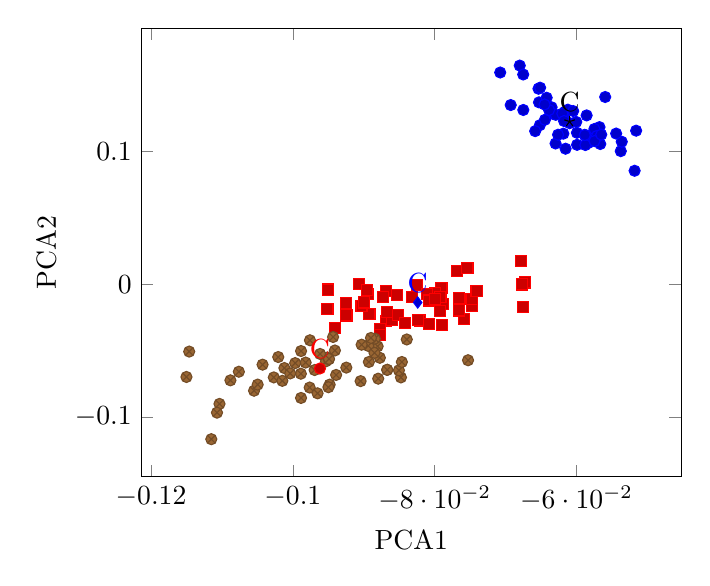
\begin{tikzpicture}
\begin{axis}[
xlabel={PCA1},
ylabel={PCA2},
]
\addplot+[
nodes near coords,
only marks,
point meta=explicit symbolic,
]
table[
meta=label,
] {
x y label
-0.06161711715313449 0.12996942830060373 $$
-0.05807229769243277 0.11137145174192183 $$
-0.05676338516730648 0.1182947693033406 $$
-0.056654313968970874 0.105607729117619 $$
-0.06123006441704709 0.1314311417740595 $$
-0.06750333894965883 0.13121548909498384 $$
-0.05748191998868599 0.11688581315371398 $$
-0.060973238901847825 0.12128227872938517 $$
-0.05376213630754356 0.10023310181869789 $$
-0.058827956809018665 0.11239131256616681 $$
-0.06529216383472475 0.13695682834115136 $$
-0.059942307914473435 0.11405684263162513 $$
-0.057114464451829404 0.11170394422395846 $$
-0.05159569819216177 0.11563975235933245 $$
-0.06800666760874802 0.1646310497964307 $$
-0.07076141332462106 0.15942601962430097 $$
-0.06536411073785399 0.14721505155300138 $$
-0.06179208137357522 0.1280241630769381 $$
-0.06928116550563142 0.1349245863284467 $$
-0.0635143372787522 0.13324773110768848 $$
-0.06517432908840144 0.11973358846688771 $$
-0.06329348521511752 0.12822797966893926 $$
-0.055959360124591025 0.14097961326556566 $$
-0.06295479840515956 0.10598498835592639 $$
-0.061546729073327096 0.10205717078811198 $$
-0.05992478081849803 0.10498444325454095 $$
-0.0618579743956802 0.11339185766755219 $$
-0.06293479322624863 0.1275823104277258 $$
-0.06200416988922219 0.12850771482714526 $$
-0.058367806326160156 0.10629509745982745 $$
-0.05875485906224769 0.10483338398637032 $$
-0.06445464342338017 0.12384283924856791 $$
-0.06513472671025955 0.1479744929418998 $$
-0.06751930722231257 0.15794192277270835 $$
-0.058827956809018665 0.11239131256616681 $$
-0.05857718517484365 0.12713297814272842 $$
-0.0642137861808346 0.14042040988161797 $$
-0.058827956809018665 0.11239131256616681 $$
-0.0536231455386676 0.1073074786482872 $$
-0.0617561079220106 0.12289505147101303 $$
-0.06047440530046122 0.1304112809498146 $$
-0.05181026479074422 0.08545358266065609 $$
-0.05441477810681811 0.11345645107845713 $$
-0.06260371912063663 0.1125758134353086 $$
-0.06582852971099769 0.11530290342600667 $$
-0.05746439289271059 0.10781341377662985 $$
-0.06387418011126283 0.13119310571684845 $$
-0.056515323200094905 0.11268210594720839 $$
-0.06450929481456197 0.1353440555995235 $$
-0.06004261556482133 0.12220768312880462 $$
};
\addplot+[
nodes near coords,
only marks,
point meta=explicit symbolic,
]
table[
meta=label,
] {
x y label
-0.09505238307667932 -0.003950921216340174 $$
-0.08946051907024073 -0.007573041660762608 $$
-0.09511827609878432 -0.018583226625726007 $$
-0.07582838762646103 -0.0258683887513271 $$
-0.08919493000705372 -0.022258104393979006 $$
-0.08204724235191896 -0.027269865265168614 $$
-0.0903180446604962 -0.016056374639978613 $$
-0.06725844775757917 0.0013644909865145269 $$
-0.09002368687041061 -0.013680314989937624 $$
-0.074703202869763 -0.01635413672503065 $$
-0.0675276657473434 -0.017320462361206265 $$
-0.08315012024242258 -0.009786205955558484 $$
-0.078822023781878 -0.015043215587280065 $$
-0.08681911304298845 -0.02768933453624546 $$
-0.07684692613927042 0.010190863738827991 $$
-0.09070353857326205 1.3594618720455024e-4 $$
-0.08240593434078786 -0.026624196023955125 $$
-0.07977017421487986 -0.006896220609615304 $$
-0.07651815372094192 -0.010216222517696393 $$
-0.08767548778960216 -0.03347237288340778 $$
-0.08250468316781408 -8.193212261354083e-4 $$
-0.086073368318032 -0.02687329030400184 $$
-0.08685352767123136 -0.004906188629680096 $$
-0.089524853269024 -0.004551312769508217 $$
-0.09243818695300396 -0.02347430217443999 $$
-0.0940414572682159 -0.0327736793858996 $$
-0.08514159413736379 -0.0232475912725288 $$
-0.07538264659293452 0.012415864120698245 $$
-0.07480466136375263 -0.01090359085990477 $$
-0.07409489009036085 -0.004958435021736108 $$
-0.07905048854985862 -0.00278696982793511 $$
-0.08084019630046224 -0.029849741507210762 $$
-0.08729563977818063 -0.009820425420768301 $$
-0.0924829239525563 -0.013808990879972899 $$
-0.08423056799956825 -0.0289657692763221 $$
-0.07991677768810178 -0.00673410311860897 $$
-0.07662002019461153 -0.01971941632115717 $$
-0.07898010047005105 -0.030699227340425506 $$
-0.08668012227411244 -0.020614957706656098 $$
-0.07918947931873456 -0.009861346657524472 $$
-0.06764550049366673 -9.722248694261789e-5 $$
-0.07926413588882725 -0.019957452378368254 $$
-0.08105948954077519 -0.007175955767821258 $$
-0.08083863747714053 -0.012195707206570507 $$
-0.08528778963090575 -0.00813173411293578 $$
-0.06779054514356696 0.01771892930470396 $$
-0.07990801414011407 -0.011270302807151055 $$
-0.08766672424161445 -0.03800857257194987 $$
};
\addplot+[
nodes near coords,
only marks,
point meta=explicit symbolic,
]
table[
meta=label,
] {
x y label
-0.08393661818916259 -0.04154344929486779 $$
-0.08804616427335603 -0.046706780366002704 $$
-0.08773376810736117 -0.055341172613389285 $$
-0.09884521433282735 -0.08556233964151426 $$
-0.08669292272835737 -0.06440251376763782 $$
-0.10268605370719039 -0.07010266484458498 $$
-0.09389797144163735 -0.06824386547818649 $$
-0.09762899675370301 -0.07772467590351184 $$
-0.1103440481786629 -0.09003803543797657 $$
-0.07529669822015317 -0.05717656673810322 $$
-0.10547031101392385 -0.08011537236343891 $$
-0.09651579649188997 -0.08209050060102373 $$
-0.10761329141946953 -0.06582381693611337 $$
-0.09432705151031379 -0.03968593872448259 $$
-0.09245975095523658 -0.06272565854687961 $$
-0.09819821843489714 -0.058941420611450884 $$
-0.08475857830753342 -0.07010963354859544 $$
-0.08796356011463553 -0.07105435367087433 $$
-0.09513868925737519 -0.05513428836611204 $$
-0.09532471871308698 -0.057943943165341474 $$
-0.11500321874481956 -0.06977452881383779 $$
-0.11149800166225958 -0.11661340984753028 $$
-0.08504491541359312 -0.06476844785064541 $$
-0.10119226256999406 -0.06306998711599048 $$
-0.08462835108664517 -0.05849905703046407 $$
-0.11069512746318584 -0.09662886051735875 $$
-0.08936268950282833 -0.046393603606825685 $$
-0.09967241237286253 -0.05933051593683266 $$
-0.10427046968713315 -0.06050501461629872 $$
-0.08844082971378954 -0.04093199951886414 $$
-0.08898440031472846 -0.040395690444826465 $$
-0.09480991683904666 -0.07554137462263645 $$
-0.10205929457219903 -0.05476367537013128 $$
-0.10496271386454956 -0.07552256983155158 $$
-0.11461460718541029 -0.05065878103974042 $$
-0.09498488105948726 -0.07748663984630072 $$
-0.09030322723148426 -0.04548310294975664 $$
-0.09044492766732365 -0.0729118087120398 $$
-0.10880281037495082 -0.07231634007115535 $$
-0.09692683818465714 -0.0645430257447474 $$
-0.09493766597699944 -0.05648222969188433 $$
-0.09884209668618396 -0.05025427104023373 $$
-0.09887086541308257 -0.06731539342349097 $$
-0.09758760396821148 -0.042145129644049095 $$
-0.08669292272835737 -0.06440251376763782 $$
-0.10147900765573367 -0.0726825410866271 $$
-0.10037226925462489 -0.0671115768314898 $$
-0.09616085669676186 -0.05244505195689411 $$
-0.08928082820806965 -0.058487731875164255 $$
-0.09407022599511451 -0.0498348017691569 $$
-0.09489939083815128 -0.05621075203370223 $$
-0.08848827638030532 -0.051621017157090845 $$
};
\addplot+[
nodes near coords,
only marks,
point meta=explicit symbolic,
]
table[
meta=label,
] {
x y label
-0.06097591169212255 0.12251649653540746 C
};
\addplot+[
nodes near coords,
only marks,
point meta=explicit symbolic,
]
table[
meta=label,
] {
x y label
-0.08239273499786132 -0.013729627446612947 C
};
\addplot+[
nodes near coords,
only marks,
point meta=explicit symbolic,
]
table[
meta=label,
] {
x y label
-0.09617812168198688 -0.06337689296894312 C
};
\end{axis}
\end{tikzpicture}


